\documentclass[crop,border={0pt 0 0 0},tikz]{standalone}
\usetikzlibrary{backgrounds,decorations.markings, calc,intersections, through}
\tikzset{>=latex}
\tikzset{->-/.style={decoration={
  markings,
  mark=at position .5 with {\arrow{>}}},postaction={decorate}}}
\begin{document}
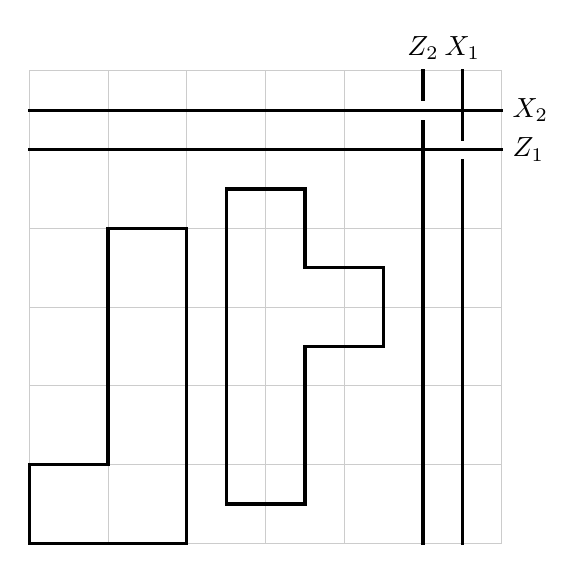
\begin{tikzpicture}
    \begin{scope}[on background layer]
        \draw [step=1, line cap = rect, gray!40] (1.0,1.0) grid (7,7);
    \end{scope}
    
    \draw[black, line cap=rect, very thick] (3.5,5.5) -- (3.5,1.5) -- (4.5,1.5) -- (4.5,3.5) -- (5.5,3.5) -- (5.5,4.5) -- (4.5,4.5) -- (4.5,5.5) -- cycle;

    \draw[black, line cap=rect, very thick] (1,1) -- (1,2) -- (2,2) -- (2,5) -- (3,5) -- (3,1) -- cycle;

    \draw[black, line cap=rect, very thick, name path=x1] (6.5,1) -- (6.5,7) node[anchor = south] {$X_1$} node[pos=0.832, fill=white, anchor=center]{};
    \draw[black, line cap=rect, very thick] (6,1) -- (6,7) node[anchor = south] {$Z_2$} node[pos=0.916, fill=white, anchor=center]{};
    \draw[black, line cap=rect, very thick] (1,6.5) -- (7,6.5) node[anchor = west] {$X_2$};

    \draw[black, line cap=rect, very thick, name path=z1] (1,6) -- (7,6) node[anchor = west] {$Z_1$};

    
    

    


\end{tikzpicture}
\end{document}
